\documentclass{uebungszettel}
\usepackage{algorithm,algorithmic}

\floatname{algorithm}{Algorithmus}
\newcommand{\SET}{\textbf{set}\ }
\newcommand{\CHOOSE}{\textbf{choose}\ }
\newcommand{\GOTO}{\textbf{goto}\ }
\renewcommand{\algorithmicrequire}{\textbf{Input:}}
\renewcommand{\algorithmicensure}{\textbf{Output:}}
\renewcommand{\listalgorithmname}{Algorithms}
\renewcommand{\algorithmiccomment}[1]{\\/* #1 */}

\newcommand{\utitle}{Tag 4}

\begin{document}
\newcommand{\ah}[2]{\ \\* \emph{(#1, #2)}\\}


\begin{aufg} Implementiere einen Graphen als Adjazenzliste mit Listen an jedem Knoten $v$ f�r $\delta^-(v)$ und $\delta^+(v)$. Implementiere mit Hilfe dieser Datenstruktur den Edmonds-Karp Algorithmus.
\end{aufg}

\begin{aufg}[$\ast$] Implementiere den Push-Relabel Algorithmus.
\end{aufg}

\vfil
\centering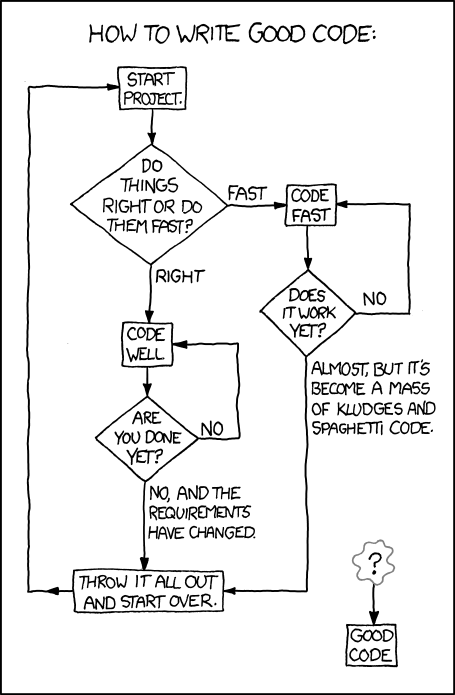
\includegraphics[width=.7\textwidth]{good_code}
\vfil~

\end{document}
